%%%%%%%%%%%%%%%%%%%%%%%%%%%%%%%%%%%%%%%%%
%%% WP01
%%%%%%%%%%%%%%%%%%%%%%%%%%%%%%%%%%%%%%%%%

\tsubsubsection{WP4 - Access to RI for Detectors}

%%%%%%%%%%%%%%%%%%%%%%%%%%%%%%%%%%%%%%%%%
%%% Section content, please change!
%%%%%%%%%%%%%%%%%%%%%%%%%%%%%%%%%%%%%%%%%

\subsubsection*{Overview and Goals}

\begin{table}[H]
    \renewcommand{\arraystretch}{1.50}		
    \footnotesize   
    \begin{tabular}{*{3}{|p{0.10\textwidth}}|l|}
        \hline
        \rowcolor{mygray} \multicolumn{4}{|c|}{\textit{\color{white}Work Package Summary}} \\
        \hline
        \rowcolor{mylightergray} \textit{WP No.} & \cellcolor{white} 4 & \textit{Title of WP} & \cellcolor{white}  (TA3): Access to Research Infrastructures for Detector R\&D \\
        \hline
        \rowcolor{mylightergray} \textit{Start} & \cellcolor{white} M1 & \textit{End} & \cellcolor{white} M48 \\
        \hline
        \rowcolor{mylightergray} \multicolumn{4}{|p{0.978\textwidth}|}{\textit{Participating Organisations}} \\
        \hline
        \multicolumn{4}{|p{0.978\textwidth}|}{
            \hspace*{-0.75cm} 
            \begin{minipage}[t]{\textwidth}
    			\begin{itemize}
    			    \item WP Leader: 4 JSI
    				\item Participants: CERN, DESY, JSI, IFJ-PAN, UCL, RBI, ITAINNOVA, PSI, UoB
    			\end{itemize} 
    			\vspace*{0.10em}
			\end{minipage}
        } \\
        \hline
    \end{tabular}
    \vspace{0.5em}\vfill
    \begin{tabular}{|p{0.978\textwidth}|}
        \hline
        \rowcolor{mylightergray} \textit{Goals} \\
        \hline
        \rowcolor{white} 
        \hspace*{-0.75cm} 
        \begin{minipage}[t]{\textwidth}
        {\leftskip=15pt
        This work package provides access to world-class research infrastructures needed to carry out research and development of innovative HEP detectors required in the next generations of HEP experiments.
    		\begin{itemize}
    		    \item Task 4.1 TA to test beam facilities - coordinated by CERN
    			\item Task 4.2 TA to detector characterization facilities - coordinated by ITTAINOVA
			    \item Task 4.3 TA to Irradiation facilities - coordinated by CERN
                    \item Task 4.4 Service improvements - coordinated by JSI
    		\end{itemize} 
    		\vspace*{0.10em}
        }
	\end{minipage}        
        \\
        \hline
    \end{tabular}
    \vspace{0.5em}\vfill
    \resizebox{\textwidth}{!}{%
    \begin{tabular}{|l|*{8}{>{\centering\arraybackslash}p{0.084\textwidth}|}}
        \hline    
        \rowcolor{mylightergray} \textit{Participant number} & \textit{1} & \textit{2} & \textit{3} & \textit{4} & \textit{5} & \textit{6} & \textit{7} & \textit{8}\\
        \hline
        \rowcolor{white} \cellcolor{mylightergray}\textit{Participant short name} & JSI & CERN & DESY & IFJ-PAN & UCL & RBI & ITAINNOVA & UoB \\
        \hline
        \rowcolor{white} \cellcolor{mylightergray}\textit{PM per participant~\footnotemark} & 18 & 82 & 16 & 11 & 3 & 8 & 17  & 18.1 \\
        \hline        
    \end{tabular}
    }
\end{table}
\footnotetext{the PM figures correspond to the full duration of the project.}
\subsubsection*{Status}
WP4 of EURO-LABS is devoted to support detector R\&D via Transnational Access (TA) carried out at 11 RIs in Europe. The typical detector R\&D cycle consists of constructing a series of prototypes, testing them in high-energy particle beams, irradiating them and possibly evaluating their performance in special characterization facilities. This is followed by the division of WP4 into tasks: 
\begin{itemize}
    \item WP4.1 supplies the test beams in 3 RIs, 
    \item WP4.2 offers detector characterization in 2 RIs and
    \item WP4.3 irradiation opportunities in 6 RIs.
\end{itemize}

The three RIs offering test beams in WP4.1 are:
\begin{itemize}
    \item 4.1.1: CERN PS and SPS test beams,
    \item 4.1.2: DESY-II Test beam Facility,
    \item 4.1.3: PSI PiM1 and UCN test beams.
\end{itemize}

The \textbf{CERN} PS (Proton Synchrotron) and SPS (Super Proton Synchrotron) test beams provide particle beams in the energy range from ~1 GeV to ~350 GeV. Upstream of the physicist’s test setup sophisticated beam line equipment allows selecting the type, polarity and energy of particles as well as the beam intensity. A total of seven general purpose test beam lines and their large, well-equipped experimental areas are available for detector R\&D.

\textbf{DESY} (Deutsches Elektronen-Synchrotron) at Hamburg presently operates several particle accelerators of worldwide relevance including PETRA III, FLASH and the European XFEL. The DESY II synchrotron is used as an injector for PETRA III and delivers in parallel electron or positron beams for up to three test beam areas using a fixed secondary target. As the demand on the PETRA III light source is high, DESY II operates with a very high availability of >99\%. DESY II can provide electron beams with an energy between 1 GeV and 6 GeV, a small energy spread of about 5\%, and rates up to several 10 kHz, depending on beam line and the choice of the secondary target. 

The Paul Scherrer Institut (\textbf{PSI}) is a multidisciplinary Swiss national research laboratory. Among other accelerators it runs the high intensity proton accelerator (HIPA) complex which delivers protons to the Swiss research infrastructure for particle physics (CHRISP). Both installations of WP4.1.3, PiM1 and UCN, belong to CHRISP and serve both, physics experiments and test beam areas for detector qualification. The secondary beamline PiM1 is designed to provide pions with a very well-defined momentum between 100 and 500 MeV/c. However, also a beam operation mode for electrons and muons exists. The beam profile and particle flux are adjustable by the users. The beam is continuous with a bunch frequency of 50MHz. The ultracold neutron facility (UCN) has 2 beamlines (West-1, West-2). West-1 provides a world-leading UCN intensity and is operated in a pulsed mode with UCN pulses every 300s, or at adjustable longer intervals or lower intensity on user request. West-2 provides about a factor 10 lower intensity. 

The two RIs offering detector characterization in WP4.2 are:
\begin{itemize}
    \item	4.2.1: RBI-AF, Croatia,
    \item	4.2.2: ITAINNOVA EMC Lab, Spain.
\end{itemize}

Ruder Boskovic Institute (\textbf{RBI}) runs the Tandem accelerator facility (RBI-AF) used for experiments in nuclear physics and applications. RBI-AF is equipped with 1 MV Tandetron and 6 MV EN Tandem accelerators and 9 end-stations, including two ion microbeams, end station for Time-of-Flight Elastic Recoil Detection Analysis (TOF-ERDA), end-station for ion channeling experiments, large vacuum chamber for ion irradiation experiments, etc. Ion microbeam stations have multifunctional capabilities, including ion irradiations at microscopic scale and the use of ion beams as a probe for detector characterization studies using for example Ion Beam Induced Charge technique (IBIC). This facility is a key instrument for detector characterization at microscopic scales. RBI-AF has been regularly used by many international research groups for various applications, including detector characterization, mainly by exploiting the IBIC and TRIBIC techniques and irradiation by MeV ions for radiation hardness studies. 

The Instituto Tecnológico de Aragón (\textbf{ITAINNOVA}) is a non-profit Research and Technology Organisation (RTO). The EMC lab is fully equipped to perform any EMC measurement. Two
semi-anechoic chambers and Faraday cage allow to carry out standardized EMC tests as well as EM characterization of mid-scale prototypes. The lab is an accredited laboratory for European Directive and several product standards. The laboratory has several current probes to measure and inject conducted noise from DC up to 400 MHz, antennas to measure noise from few kHz up to 18 GHz and inject noise with generators up to 20 GHz and amplifiers up to 6 GHz.

The six RIs offering irradiations in WP4.3 are:
\begin{itemize}
    \item	4.3.1: CERN IRRAD, Switzerland,
    \item	4.3.2: CERN GIF++, Switzerland,
    \item	4.3.3: JSI TRIGA reactor, Slovenia,
    \item	4.3.4: IFJ PAN AIC-144 cyclotron, Poland,
    \item	4.3.5: UCLouvain CRC, Belgium,
    \item	4.3.6: UoB MC40 Cyclotron, United Kingdom.
\end{itemize}

The goal is to cover the wide range of identified particle sources needed for detector development for later stages of High Luminosity LHC (HL-LHC) upgrades and enable initial research on detectors for the Future Circular Collider (FCC). These RI’s include proton, neutron or mixed field sources as well as gamma irradiation. Some can provide extreme fluences beyond 10$^{17}$ n$_{eq}$/cm$^2$ (JSI, IFJ-PAN, UoB) for smaller samples, while others deliver lower fluences of ~10$^{15}$ n$_{eq}$/cm$^2$ on larger (10x10 cm$^2$) objects. GIF++ covers irradiation of large-scale objects like muon chambers, while the Heavy Ion Irradiation Facility (HIF) at UCL is widely used for Single Event Effect tests of electronics. 

The operational parameters of the irradiation RIs are summarized in the following table:

    \begin{tabular}{|l|*{8}{>{\centering\arraybackslash}p{0.1\textwidth}|}}
        \hline    
        \rowcolor{mycyan} Infrastructure % short name
        &Sub-task number & Installation name & Source & Particle & Energy [MeV] & ${\phi}_{max}$ part s$^{-1}$cm$^{-2}$\\
        \hline
        \rowcolor{white} CERN & 4.3.1 & IRRAD & PS & Protons & 24000 & 10$^{10}$ \\
        \hline
        \rowcolor{white} CERN & 4.3.2 & GIF++ & $^{137}$Cs & Gamma & 0.662 & 14 TBq  \\
        \hline
        \rowcolor{white} JSI & 4.3.3 & Triga Mark III & Reactor & Neutrons & <10 (Watt spectrum) & 7x10$^{12}$  \\
        \hline
        \rowcolor{white} IFJ-PAN & 4.3.4 & AIC-144 Cyclotron & Cyclotron & Protons & 10-60 & 3x10$^{11}$  \\        
        \hline       
        \rowcolor{white} UCLouvain & 4.3.5 & CRC NIF, LIF, \hspace{12pt} HIF & Cyclotron & Neutrons, Protons, Heavy Ions & <50(cont.) 10-62 110 Q$^2$/M & 7x10$^{10}$ 2x10$^{8}$ \hspace{6pt} $10^{4}$ \\
        \hline        
        \rowcolor{white} UoB & 4.3.6 & MC40 Cyclotron & Cyclotron & Protons & 26 & 1.5x10$^{13}$  \\
        \hline        
    \end{tabular}

\subsubsection*{Reports from WP4 RIs}

\subparagraph{Sub-task 4.1.1 CERN PS\&SPS} \mbox{}

The PSSPS facility at CERN provides multiple test beams opportunities for users, including three general purpose beam lines adjacent to the PS accelerator complex in the so-called East Area (T9 and T10 for general applications, T11 for activities compatible with the existing fixed installation of the CLOUD experiment) and four general purpose beam lines supplied by the SPS accelerator in the so-called North Area (H2, H4, H6, and H8). An example of a typical experimental area on one of the EHN1 beam lines can be seen in Fig. \ref{fig:4.1.1} The two areas are differentiated by the beam energies that can be realized (East Area for energies in the magnitude of 10 GeV, North Area for energies in the magnitude of 100 GeV). The East Area has been renovated and improved during the LS2 long shutdown and resumed, together with the North Area, operation again in June 2021. Starting with September 2024, another test beam line belonging to the PS accelerator complex has been added. This TELMAX line is dedicated to research and development in the field of anti-matter research and is hosted on premises of the “Antimatter Factory” as part of the AD and ELENA infrastructure at CERN. 

\begin{figure}[!h]
    \centering
    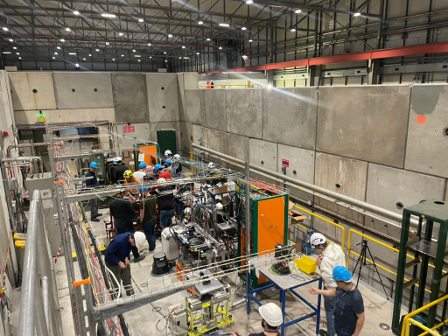
\includegraphics[width=0.75\linewidth]{image.png}
    \caption{Installation of a user experiment in one of the experimental zones on the H8 beamline in the EHN1 building.}
    \label{fig:4.1.1}
\end{figure}

Overall, demand for beam time in our facility is very high and the PS \& SPS Physics Coordinators receive requests from about 100 – 120 different activities for beam time per year from users all over the world. The utilization of the machines is generally above 100\% due to the infrastructure allowing multiple experiments to occur in parallel to each other in several experimental zones (with the new TELMAX beamline not being used to the full capacity yet).

To support the PS \& SPS Physics Coordinators in organizing and handling the requested beam times and manage the user schedule over all beamlines and experimental zones of the facility, a software solution has been developed under the WP 4.4.1 service improvement program. This user schedule management tool was first used for the beam requests in the 2023 beam period and has since then been expanded and integrated into the workflow of user request and change management, reporting of statistics, handling of short-term cancellations and overall communication with the users of the PSSPS facility. Development and maintenance of the tool at least until the end of the beam period in August 2026 has been secured, with additional efforts to investigate opportunities and synergies including a tighter integration and consolidation with other similar management tools at CERN also being investigated and explored. 

Since the start of the project and until the end of reporting period P2, a total of 57 projects applied for funding under the trans-national access (TA) scheme, representing 16004 access units (AU) of delivered beam time in the PSSPS facility and a funding request for a total of 284 users. This represents an increase compared to the numbers for the end of the P1 period (30 projects, 9072 AU, 164 users) of 28 projects, 6932 AU and 120 users. The numbers of P2 also include the first successfully granted application of a user in the new TELMAX beamline. 

Within the objectives and constraints of the WP4 efforts, it was expected that the number of TA applications would decline rather sharply over the runtime of the project. This is due to the high number of activities being associated with the four large LHC experiments, with many of their activities targeting an installation into their respective detectors during the upcoming LS3 shutdown of the CERN accelerator complex. Those activities were expected to mostly transition from R\&D to calibration and quality assurance tasks during reporting periods P2. However, the overall schedule at CERN did change and, with the extension of beam activities until August 2026 and subsequent shift of the LS3, R\&D test beam activities for the LHC experiments targeting installation in LS3 have continued throughout 2024 and, at a significantly decreased rate, are also expected to continue throughout 2025. Additionally, activities targeting subsequent shutdowns (i.e., LS4 or later) and also a number of activities unrelated to the development of LHC detector subsystems continue to perform R\&D tasks. For example, activities under the umbrella of the DRD collaborations are especially worth mentioning here, with first TA applications (3 visits, 936 AU,  13 users) for these groups of users having been filed for the reporting period during 2024. It is therefore expected that the decline in TA applications will be more gradual and less steep than initially anticipated. 

\subparagraph{Sub-task 4.1.2 DESY} \mbox{}

The DESY test beam facility operates at the DESY-II accelerator and is equipped with three test beam lines, providing up to 1,000 particles per cm² with energies from 1 to 6 GeV, an energy spread of ~5\% and a divergence of ~1mrad. Access to these beam lines coupled with extensive technical and administrative user sort is the main objective in the EURO-LABS Transnational Access programme at DESY (WP4.1.2). 

\begin{figure}[!h]
    \centering
    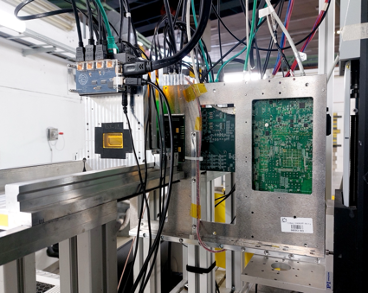
\includegraphics[width=0.75\linewidth]{image2.png}
    \caption{Set-up with RD50-MPW4 D-MAPS CMOS sensor in the DESY II test beam facility. Performance of detectors before and after irradiation was evaluated and compared with results from the previous submission.}
    \label{fig:4.1.2}
\end{figure}

During the second reporting period of the project, 13 user groups with a total of 59 users from 13 different countries have applied for TA. All TA-applications have been approved by the USP. All international teams have been granted in total with 2832 beam-hours of transnational access. 

To ensure the most efficient and transparent support for the user a new automated administrative procedure has been rolled out and is presented in detail on the webpage EURO-LABS at DESY. The processing time for applications and reimbursements has been improved, ensuring timely coverage for all users.

In P1 and P2 of the project, international teams that requested TA support have been granted 4704 beam-hours (AUs) of transnational access in total. 22 projects with a total of 97 users (80 users were funded) from 14 different countries have been granted TA.

\subparagraph{Sub-task 4.1.3 PSI} \mbox{}

The EURO-LABS project in Switzerland could only be started in 2023 as the funds for TA support needed to be confirmed by SERI (State Secretariat for Education, Research and Innovation). The first 4.5 month of the beam period in 2023 were dedicated to a physics experiment, MUSE. Test beams were scheduled for the time after October. Only 2 teams doing test beams applied for TA support: COMET and a group from Mainz and Heidelberg. 

\begin{figure}[!h]
    \centering
    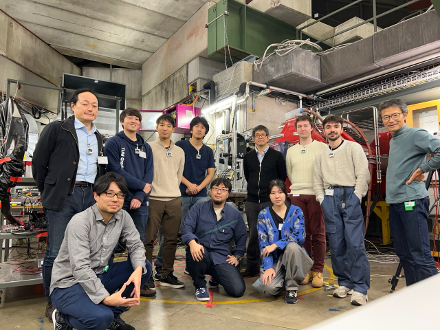
\includegraphics[width=0.75\linewidth]{image3.png}
    \caption{Members of the COMET test beam team at the PiM1 line in PSI, their set-up in the background.  }
    \label{fig:4.1.3}
\end{figure}

The COMET experiment will search for the muon-to-electron conversion process at J-PARC, Japan. This project will primarily involve negative pions, muons, and electrons with a momentum of <200 MeV/c. The primary objective of the test beam was to scrutinise the secondary particles emanating from tungsten blocks, subjected to pions and muons. This analysis was facilitated by a set of plastic scintillating counters. Both tested detectors will contribute to the particle-type identification of these secondary particles. In addition, two COMET detectors, the Range Counter and a prototype of the Cylindrical Trigger Hodoscope were also tested with muon beams in parallel. Those results have also independently contributed to the development of the COMET experiment. 

The group consisted of 12 scientists from Japan, France, and the UK. Five of them - all PhD students - were supported in the framework of the EURO-LABS project.

The second group supported tested a very compact spectrometer consisting of a four-layer pixel detector and a strong permanent neodymium dipole magnet.  This setup serves as a demonstrator for a "photon tracker", where the conversion electron positron pair is tracked in double layers of pixel detectors. The pixel tracker is based on MuPix sensors developed for the Mu3e experiment.

The project was granted two weeks of beam time. Four undergrad-students form the Universities of Heidelberg and Mainz obtained TA support.

In 2024 the schedule was similar to 2023. The PiM1 beam line was dedicated to the MUSE experiment up to mid-August and from the second half of October. Test beams are only scheduled for the time in-between. Several groups have applied for TA funding. Up to end of P2, a total of 11 projects with 32 users were executed, consuming a total of 2808 AUs.

\subparagraph{Sub-task 4.2.1 RBI} \mbox{}

The Tandem Accelerator Facility at the Rudjer Bošković Institute (RBI-AF) is one of the two facilities within the task 4.2 Detector Characterization of WP4. At RBI-AF users can perform:
\begin{itemize}
    \item	in vacuum and in-air IBIC (Ion Beam Induced Charge) imaging of charge collection properties using protons of up to 10 MeV with 1 $\mu$m resolution and heavy ions on demand and/or time resolved IBIC (TRIBIC),
    \item	radiation hardness studies with real-time controlled radiation damage of small detector area using protons or heavier ions, including ion beam analysis.
\end{itemize}
For such studies users can use two ion microprobe end-stations and other end stations, depending on the actual objectives of the proposed work.

In one of the performed TA user projects charge transport response of SiC sensors to harsh environments and to single ion implantation has been studied. The experiment was mostly focused on characterization of world’s first in-line sensor for single ion implantation applications. In the experiment unique capabilities for deterministic heavy ion counting of the novel ultra-thin SiC radiation detectors realized by STLab srl were investigated by users from Switzerland and Italy.

Detailed 3D charge collection efficiency (CCE) characterization of large area single pad SiC detectors dedicated to the use for the particle identification by the MAGNEX focal plane detector within the NUMEN project (double beta-decay study) at LNS Catania were investigated by users from Italy.

CCE characterization of position sensing photodiodes as detectors to determine the impact position of monoenergetic MeV ions was the next subject studied. The spatial resolution and radiation hardness of this position sensitive detector has been characterized by the analysis of experimental data supported by a suitable theoretical model. 

The behaviour and resulting concentration in depth profiles of MeV 7Li ions implanted in novel commercial detector crystalline materials, such as artificial diamond and SiC polytypes was studied. The implantation has been carried out in the axial channeling mode. 

High temperature implantation of Group IV elements into diamond was investigated. Group IV defects in diamond offer a promising platform for applications in quantum technology, quantum sensing and device fabrication, including magnetic field sensors and quantum thermometry. 

\begin{figure} [!h]
    \centering
    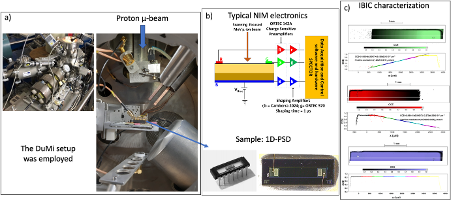
\includegraphics[width=0.75\linewidth]{image4.png}
    \caption{Experiment for the characterization and modification of a 1D-PSD. a) The experiment was carried out at the Dual Microprobe (DuMi) end-station, b) the detectors were read out with NIM-based electronic units, c) IBIC (Ion Beam Induced Charge) microscopy was carried out. After characterization, the detector was modified by means of controlled irradiations aiming to obtain a 2D-PSD response.}
    \label{fig:4.2.1}
\end{figure}

\subparagraph{Sub-task 4.2.2 ITAINNOVA} \mbox{}

During this period, CEA-Saclay requested access to perform a series of tests aimed at characterizing and evaluating the noise susceptibility of the Front-End Electronics (FEE) and DAQ system (ARC) used in the IAXO experiment. ARC currently serves as the reference design for the RadioPure version of the FEE. The IAXO experiment targets the detection of axions in the low-energy range of the spectrum. This requires the MicroMegas detector, the analog signal conditioning stages, and the DAQ system to operate under extremely low electromagnetic noise conditions. Previous issues in IAXO - electronics prototype highlighted the need for this study. Several test campaigns were carried out at EMCLab to support the integration of the improved RadioPure ARC, as shown in Fig. \ref{fig:4.2.2}.

\begin{figure}[!h]
    \centering
    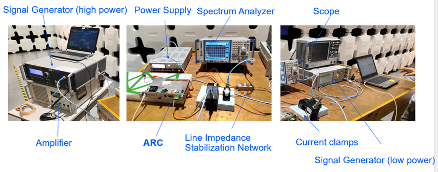
\includegraphics[width=1\linewidth]{image5.png}
    \caption{Detail of the characterization setup of the ARC DAQ in the anechoic chamber.}
    \label{fig:4.2.2}
\end{figure}
The characterizations reported a good immunity of the ARC to conducted noise in the power lines of the electronics. The topological placement of the ASICs in the PCB showed small differences in noise coupling, i.e. noise transfer function (TF) differences between chips. The TF of the input channels has also been studied, enabling the operation of the input stages of the conditioning ASIC in configurations that filter noise for different frequency regions of the input spectrum as it is shown in Fig. \ref{fig:4.2.2a}. The study reports the tunning capabilities of the configuration parameters of the DAQ to cope the noise characteristics at the possible locations where the experiment is studied.

\begin{figure}[!h]
    \centering
    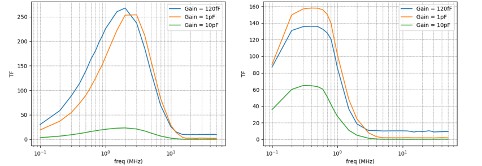
\includegraphics[width=0.75\linewidth]{image6.png}
    \caption{Frequency response of the ARC input for a shaping time of 70 ns (left) and 640ns(right) and different gains on the feedback path.}
    \label{fig:4.2.2a}
\end{figure}
The analogue signal stages prior to the DAQ have been identified as a significant source of noise coupling, with a more pronounced impact than that observed from the DAQ itself. This highlights the need for robust shielding continuity across the entire system, particularly in the Limandes. Several design improvements have already been identified for both the Limandes and the MicroMegas to address this. These findings provide valuable insights for improving the current commissioning of the RadioPure version of the ARC and the detector setup. 

It is important to note that these recent tests have greatly benefited from the latest upgrades. They utilized new tools at the EMCLab, including a Graphical User Interface (GUI) and an automated transfer function (TF) measurement system capable of scanning the setup under various noise and configuration conditions. The tests also confirmed the adaptability and straightforward integration of the GUI and automation with different Front-End Electronics and experimental setups. This is especially relevant as IAXO uses a different hardware system compared to previous experiments tested in the EMCLab, which were primarily focused on CMS-Pixel detectors. 

To date, only three requests for access have been submitted and completed, which represents about 30\% of those initially planned. Although part of the delay is due to the early implementation of technical improvements - planned from the beginning of the project - there has also been a notable slowdown in the submission of new applications. Despite a major promotional effort to highlight the laboratory's capabilities and growing interest in launching new test campaigns, progress has been limited. Two additional applications are currently being prepared, but delays in other projects and the lack of definition of upcoming detector R\&D activities continue to slow down the formalization of new access applications.

\subparagraph{Sub-task 4.3.1 CERN IRRAD} \mbox{}

The proton irradiation facility (IRRAD) at the PS East Area (EA) was built during the Long Shutdown 1 (LS1, 2013-2014) and improved during the LS2 (2019-2021) to cope with the increasing needs for radiation tests of the experimental community working for the HL-LHC upgrade and beyond. The IRRAD facility, operated by EP-DT and exploiting the 24 GeV/c PS proton beam, is part of a more complex infrastructure that includes on the EA-T8 beamline the mixed-field facility CHARM operated by the BE department, the CERN Shielding Benchmark Facility (CSBF test station to benchmark the efficiency of radiation shielding materials), as well as serves as a test bench for developing a high-energy ion beam aiming to provide an optimal tool to reproduce the effects of galactic cosmic rays (within the HEARTS EU-funded project fostered by the CERN-ESA collaboration).

The year 2024 has been the third full year of IRRAD operation after the LS2, 30 user experiments were executed, involving more than 640 samples. About 60\% of the experiments belonged to the CERN LHC Experiments users working to complete the phase II upgrade projects, while the remanet 40\% belonged to CERN equipment groups (ATS), as well as to users from EU/R\&D/external projects. Nine out of the 30 user experiments were performed within the EUROLABS TA framework. Cumulating the EUROLABS TA projects from September 2022 to the end of 2024, a total of 3427 Access Units were provided to 13 selected projects with 32 participating users. With the strong increase of experiments performed in the TA context in 2024, the facility reached already 85\% of the overall pledged EUROLABS Access Units (AUs). The facility is expected to be fully charged in 2025 covering further EUROLABS AUs in parallel to the ongoing radiation hardness and qualification testing for components and detector elements for the HL-LHC various other projects.

\begin{figure}[!h]
    \centering
    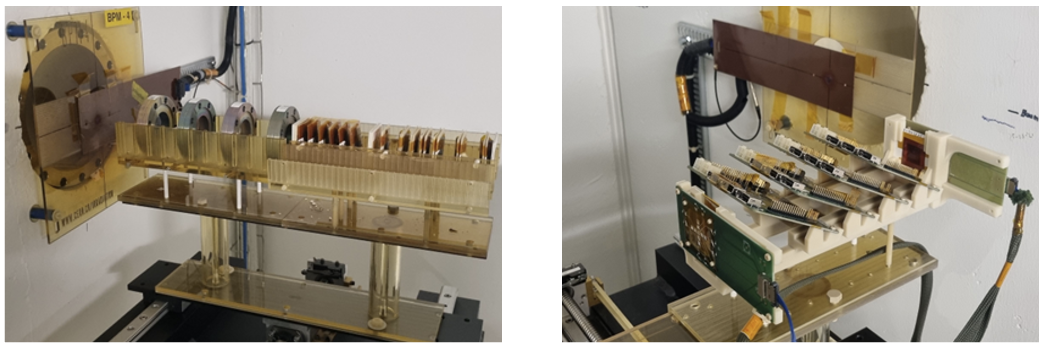
\includegraphics[width=1\linewidth]{image7.png}
    \caption{Examples of experiments performed during the run in 2023 at the IRRAD Facility. Vacuum window samples (left-hand side) and silicon pixel modules (right-hand side).
}
    \label{fig:4.3.1}
\end{figure}

Within the EUROLABS TA framework in P1 and P2 from September 2022 to February 2025 a total of 3247 Access Units were provided to 13 selected projects with 32 participating users. All-in-all, the facility is fully committed in 2025 and 2026 with the EUROLABS TA access. 

\subparagraph{Sub-task 4.3.1 CERN GIF++} \mbox{}
The CERN Gamma Irradiation Facility (GIF++) is a joint BE \& EP Department facility located on the H4 beamline (SPS, Zone PPE-154) in EHN1 hall (North Area, Prevéssin site). It is a unique place for detector R\&D, where a strong $\gamma$-ray source and a muon/pion particle beam 
are simultaneously available. Together with IRRAD in the East Area (Meyrin site), GIF++ delivers essential services to the HEP community, with the focus on validating and optimizing detector technologies, mainly in view of the High-Luminosity upgrade of LHC and accelerator projects beyond.

The irradiator (137Cs, 14 TBq as of 2014) is operated throughout the year, independently of 
the SPS and offers two adjustable gamma irradiation zones, with a total floor space of more than 100 m2 and it is expected to continue, with some limitation, also during the incoming Long Shutdown 3 (LS3). In 2024 the irradiator underwent major corrective/preventive maintenance in order to assure smooth operation over, at least, the next 5 years. A new maintenance contract was also funded and signed. 

\begin{figure}[!h]
    \centering
    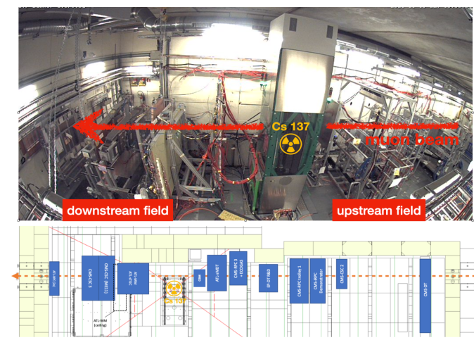
\includegraphics[width=0.75\linewidth]{image8.png}
    \caption{Photograph of the GIF++ irradiation bunker. Up to 11 different setups – often composed of multiple chambers – can be hosted along the muon beam, while several other experiments continue to use the irradiator only. The drawing at the bottom describes the experiments in the experimental area and shows the two opening cones of the gamma irradiator (downstream and upstream fields). }
    \label{fig:4.3.2}
\end{figure}

The two gamma fields (<= 2Gy/h) enable ageing studies and provide radiation background similar to the future working conditions inside the large LHC experiments. The muon (or pion) beam, available during dedicated time slots (typically 3 x 2 weeks/year) is used to investigate and validate the detector performance and behaviour under the expected conditions. During the rest of the year, for about 6 months, the facility is operated using the gamma source alone.

Several groups/set-ups are operated in parallel to optimize/maximize the use of the facility, which is equipped with excellent gas and electronics infrastructures, a unified control/monitoring system, setups for beam and cosmic trigger as well as radiation and environmental conditions monitoring.
The facility is extensively exploited by a large community, mainly composed of users belonging to the CERN LHC experiments. On average, 5 - 6 setups run continuously in parallel during the year, with a peak of 12 setups. In 2024 a campaign to validate the mass production of Resistive Plate Chambers (RPC) for the upgrade of the CMS experiment was started. Discussions are ongoing in order to enlarge the available surface in the bunker.

The extension of the gas area was approved in 2024 and will start in April 2025 to accommodate additional gas systems to cope with the increasing number of user requests. The main detector R\&D programme remains the upcoming upgrade of the LHC experiments in view of the High Luminosity LHC phase (HL-LHC), including long term ageing studies for various gas mixtures, including environmentally friendly ones. 
Over the last years the search for environmentally friendly gas mixtures gained momentum 
and became a driving element of the scientific programme of the facility via the ECOGAS collaboration.

Projects running in the facility require, with a few exceptions, long-term, even years of irradiation and scientists involved spend a large fraction (>50\%) of their working time or are permanently based at CERN.

\subparagraph{Sub-task 4.3.3 JSI} \mbox{}

The reactor facility is used for neutron irradiation to study radiation effects in particle detectors and electronics. The TRIGA reactor provides a unique opportunity for irradiation tests with neutron fluences spanning over many orders of magnitude (Fig. \ref{fig:4.3.3}). For example, electronic circuits containing COTS components were irradiated to 10¹² n/cm², while 3D detector structures were irradiated up to 10$^{18}$ n/cm².

\begin{figure}[!h]
    \centering
    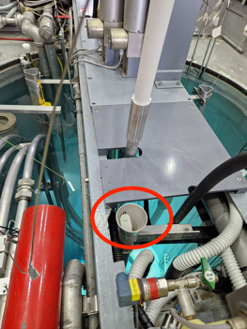
\includegraphics[width=0.6\linewidth]{image9.png}
    \caption{Insertion of samples into the F19 channel (encircled in red) leading to the reactor core faintly visible at the bottom of the water tank. The sample holder can be seen attached to the fishing rope used to lower it for irradiation and then lift it to a shielded position above the core for initial cool-down.}
    \label{fig:4.3.3}
\end{figure}

Since the start of EURO-LABS, 34 projects, totaling 366 Access Units (AU), have been approved by the User Selection Panel. Of these, 31 projects, accounting for 323 AU, were completed by the end of February 2025.

Several projects focused on radiation testing of detectors and electronics for High-Luminosity LHC upgrades. However, the majority were related to the development of charged particle detectors for future applications. These projects included the irradiation of various semiconductor materials such as Si, SiC, GaN, and diamond. Various device types were irradiated – from samples of bulk material (not processed), simple pad diodes to more complicated structures such as 3D detectors, SiPMs, LGADs, AC-LGADs, nLGADs, CMOS DMAPS etc.

A dedicated 120 AU irradiation campaign was organized to expose samples to the extreme fluence of 10$^{18}$ n/cm², to support the development of tracking detectors for future hadron colliders, like FCC-hh. Since irradiation at such high fluences requires significant time and cannot be repeated frequently, a joint irradiation campaign was organized. Samples from twelve institutions were irradiated together over five consecutive days. The high fluences resulted in significant radio-activation, requiring special handling and long cool-down times. Nevertheless, most samples were successfully distributed to test sites, and initial results have already been presented at meetings and conferences. The experience gained in this campaign will be invaluable for the next high-fluence irradiation, which we are planning for this or next year.

\subparagraph{Sub-task 4.3.4 IFJ-PAN} \mbox{}

The AIC-144 cyclotron facility offers 60 MeV proton beams with intensity up to 100 nA in two experimental rooms: a) the former proton therapy eye-treatment room with the setup for precise positioning and clinical-quality irradiation with beam diameters up to 40 mm and b) an experimental hall with an irradiation line equipped with 2D scanner (EURO-LABS service improvement), which allows to expose larger elements with sizes up to 400 mm x 400 mm. It is a user facility, which provides beams for experiments in detector physics, medical physics, cosmic industry and radiobiology. The irradiation stations are equipped with all type of dosimetry tools and are metrologically connected to the Secondary Standard Dosimetry Laboratory in Warsaw.

\begin{figure}[!h]
    \centering
    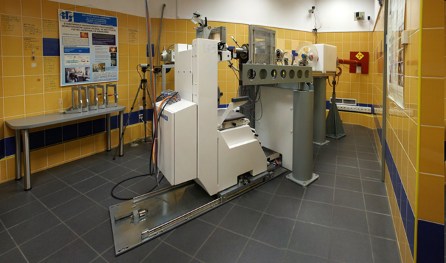
\includegraphics[width=0.75\linewidth]{image10.png}
    \caption{The irradiation room adapted from the proton therapy eye-line installation at IFJ-PAN Krakow. The samples for irradiations are mounted and positioned on the movable treatment chair in front of the beam collimator.}
    \label{fig:4.3.4}
\end{figure}

Within the EURO-LABS project, the facility was mainly used to test detectors intended for use in various experiments in physics and in space. Low gain avalanche detectors (LGAD) were tested for on-line measurements of charged particle flux with high speed and spatial precision. Further projects involved electronic modules of the POLAR-2 Gamma-Ray Burst experiment, Double Sided Silicon Strip Detectors (DS-SSD) for nuclear physics experiments, ion detector systems used for the 10 PW laser-nuclear experiments at ELI-NP and others.  Finally, silicon detectors were irradiated for studies of the defect formation and evolution. These experiments contributed to optimizing silicon detector designs and improving predictions of their behavior for future HEP applications.  Since the start of EURO-LABS 9 projects were supported with 296 access units (cyclotron hours) by EURO-LABS TA.

\subparagraph{Sub-task 4.3.5 UCLouvain} \mbox{}

Cyclotron Research Centre (CRC) is a research unit attached to the Institut de Recherche en Mathematique et Physique (IRMP) at UCLouvain. The facility operates the CYCLONE110 cyclotron, able to accelerate charged ions to kinetic energies up to 110x(Q$^2$/M) MeV. Main activities of the centre are industrial applications (membrane production), and irradiation of electronic components. In total, around 2,500 effective hours of beam are delivered to users during 35 weeks of operation. Around 10\% of access is devoted to scientific applications, mainly nuclear physics experiments, detector irradiations, rad-hard electronic devices and biomedical applications.

\begin{figure}[!h]
    \centering
    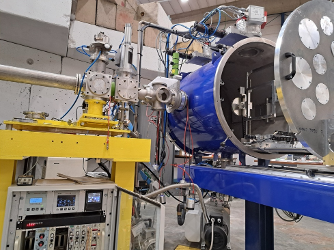
\includegraphics[width=0.75\linewidth]{image11.png}
    \caption{The end of the HIF beam line with the newly installed test chamber }
    \label{fig:4.3.5}
\end{figure}

CRC offers 3 irradiation facilities based on CYCLONE110 operation:
\begin{itemize}
    \item Neutron Irradiation Facility (NIF). Neutrons obtained impinging a 50 MeV deuteron beam on a Be target giving a continuous neutron spectrum up to 50 MeV with a mean energy of 20 MeV. The intensity of the beam can reach a flux of 7.3x10$^{10}$ n s$^{-1}$cm$^{-2}$, providing a beam diameter ~4 cm. Irradiation area can be maintained at constant temperature down to -20$^{\circ}$C during irradiation.
    \item Light Ion Irradiation Facility (LIF). Mono-energetic protons with energies between 20 and 65 MeV. Beam size of ~8 cm diameter and maximum flux of 5x10$^{8}$ p s$^{-1}$cm$^{-2}$.
    \item Heavy Ion Irradiation Facility (HIF). This facility provides a beam of up to 10$^4$ ions s$^{-1}$cm$^{-2}$ monoenergetic heavy ions with well-known range and LET. Irradiation area is ~25 mm diameter with 10\% homogeneity. Various “ion cocktails” can be accelerated allowing an easy and efficient way to change LET. The available cocktails, LET and ranges are described on the facility webpage. This facility is especially devoted to irradiating electronics. DUTs are in vacuum and must not be encapsulated. 
\end{itemize}
All these three facilities are available to EURO-LABS users. So far, for EURO-LABS, we have received just one application, with the irradiation foreseen in spring 2025. 

The installation of the new test chamber for HIF in the scope of the UCLouvain service improvement (Fig. \ref{fig:4.3.5}) has almost been completed. The only piece missing is the installation of a new, scintillator-based detector to cross-check the ion flux measurement. The material has been procured, and it is under test with heavy ions. 

\subparagraph{Sub-task 4.3.6 UoB} \mbox{}

The MC40 cyclotron at the University of Birmingham has been working as a EURO-LABS Transnational Access facility since the beginning of the project. It has delivered irradiations to four projects, and 11 users in total, out of 12 and 36, respectively, requested on the grant. The projects covered the study of radiation damage to depleted Monolithic Active Pixel Sensors, to the I3T80 technology for the development of DC/DC power regulators, to silicon sensors, including novel Low Gain Avalanche Detectors, and the study of effects of annealing on irradiated silicon sensors. 

\begin{figure}[!h]
    \centering
    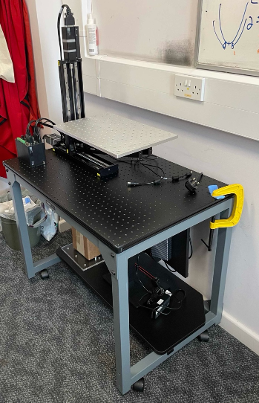
\includegraphics[width=0.5\linewidth]{image12.png}
    \caption{Upgraded sample scanning assembly during the laboratory commissioning phase. }
    \label{fig:4.3.6}
\end{figure}

By the end of the reporting period, about 30 AU were delivered, out of 300 requested on the grant. It must be noted that the MC40 cyclotron has been unavailable for approximately 6 months, between August 2022 and January 2023, due to a fire in one of the magnets that then needed replacement. During these two years, work has been ongoing on system improvements to deliver fluences well above 10$^{16}$ n$_{eq}$/cm$^2$ . The system is in the advanced stages of development (Fig. \ref{fig:4.3.6}) and is approaching a stage where commissioning at the MC40 cyclotron can begin. Full commissioning is planned in May 2025, with routine operations expected to resume in early summer 2025 with a higher fluence capability. This improvement will enable the facility to deliver a higher number of AU to projects and to work towards the delivery of the full AU target (300 AU).

\subparagraph{Task 4.4 Service Improvements} \mbox{}

The Service Improvements (SIs) task WP4.4 comprises ten improvements to facilitate user access at each of the eleven RIs of WP4. Contrary to TA, for SIs EURO-LABS resources were required to be matched by at least the same amount of funding from RIs. Also, the timeline for getting the SIs operational was set at no later than M36 of the project, with a clear preference of getting them on-line sooner to maximize their usage during the project. All but one designs of SIs are documented in their respective milestone reports; the list of SI sub-tasks with their respective target RIs and MS reports follows:
\begin{itemize}
    \item
[4.4.1]	Data base handling of beam time and irradiation requests (4.1.1 CERN TB, 4.3.1 IRRAD \& 4.3.2 GIF++) – MS24
    \item
[4.4.2]	Precision motion stages for large detector setups (4.1.2 DESY test beams) – no MS
    \item
[4.4.3]	Beam monitor (4.1.3 PSI test beams) – MS25
    \item
[4.4.4]	Ion beam focusing lens (4.2.1 RBI-AF) – MS26
    \item
[4.4.5]	Cooling System and Graphical User Interface for EMCI test station (4.2.2 ITAinnova) – MS27
    \item
[4.4.6]	Beam profile monitor (4.3.1 CERN IRRAD) – MS28, MS29
    \item
[4.4.7]	Cadmium shielding in the tangential channel (4.3.3 JSI TRIGA) – MS30
    \item
[4.4.8]	2-D scanning table for irradiation (4.3.4 IFJ-PAN AIC 144) – MS31
    \item
[4.4.9]	Test chamber for the heavy ions irradiation facility (4.3.5 UCL CRC) – MS32
    \item
[4.4.10]	Scanning system upgrade for high fluence delivery (4.3.6 UoB MC40) – MS33
\end{itemize}

\subsubsection*{Main Results and Achievements}
The usage of AUs at the eleven RIs of WP4 during P1 (Sep 22 – Aug 23) and P2 (Sep 23 – Feb 25) is summarized in Table~\ref{tabl:wp4-aunitsp1p2}.

\begin{table}[H]
    \centering
    \caption{Usage of AUs at the WP4 RIs.}
    \label{tabl:wp4-aunitsp1p2}
    \begin{tabular}{|l|*{8}{>{\centering\arraybackslash}p{0.09\textwidth}|}}
        \hline 
        \rowcolor{mycyan} WP4.1 & Name & Pledged & P1	& P2 & P1\&2	& Nominal & P1\&2/ Nominal & P1\&2/ Pledged \\
        \hline
        \rowcolor{white} WP4.1.1	&CERN 	&8736	&9072	&6932	&16004	&5460	&293\%	&183\% \\
        \hline
        \rowcolor{white} WP4.1.2	&DESY	&8640	&1872	&2832	&4704	&5400	&87\%	&54\% \\
        \hline
        \rowcolor{white} WP4.1.3	&PSI	&5376	&0	&2808	&2808	&3360	&84\%	&52\% \\
        \hline
        \rowcolor{mylightergray} Total WP4.1	& &22752	&10944	&12572	&23984	&14220	&165\%	&103\% \\
      
        \hline        
        \rowcolor{mycyan} WP4.2 & Name & Pledged & P1	& P2 & P1\&2	& Nominal & P1\&2/ Nominal & P1\&2/ Pledged \\
        \hline
        \rowcolor{white} WP4.2.1	&RBI	&504	&92	&200	&292	&315	&93\%	&58\% \\
        \hline
        \rowcolor{white} WP4.2.2	&ITAINNOVA	&800	&0	&240	&240	&500	&48\%	&30\% \\
        \hline
        \rowcolor{mylightergray} Total WP4.2	& &1304	&92	&440	&532	&815	&65\%	&41\% \\
      
        \hline   
        \rowcolor{mycyan} WP4.3 & Name & Pledged & P1	& P2 & P1\&2	& Nominal & P1\&2/ Nominal & P1\&2/ Pledged \\
        \hline
        \rowcolor{white} WP4.3.1	&IRRAD 	&4000	&1348	&2079	&3427	&2500	&137\%	&86\% \\
        \hline
        \rowcolor{white} WP4.3.2	&GIF++	&4000	&0	&3744	&3744	&2500	&150\%	&94\% \\
        \hline
        \rowcolor{white} WP4.3.3	&JSI	&700	&78	&245	&323	&437.5	&74\%	&46\% \\
        \hline
        \rowcolor{white} WP4.3.4	&IFJ PAN	&800	&80	&216	&296	&500	&59\%	&37\% \\
        \hline
        \rowcolor{white} WP4.3.5	&UCLouvain	&100	&0	&0	&0	&62.5	&0\%	&0\% \\
        \hline
        \rowcolor{white} WP4.3.6	&UoB &300	&12.5	&25	&37.5	&187.5	&20\%	&13\% \\
        \hline
        \rowcolor{mylightergray} Total WP4.3	& &9900	&1518.5	&6309	&7827.5	&6187.5	&127\%	&79\% \\
        \hline
        \rowcolor{mygray} \textbf{Total WP4	}& &\textbf{33956	}&\textbf{12554.5	}&\textbf{19321	}&\textbf{31875.5	}&\textbf{21222.5	}&\textbf{150\%}	&\textbf{94\%} \\
        \hline
    \end{tabular}
\end{table}

\begin{figure}[!h]
    \centering
    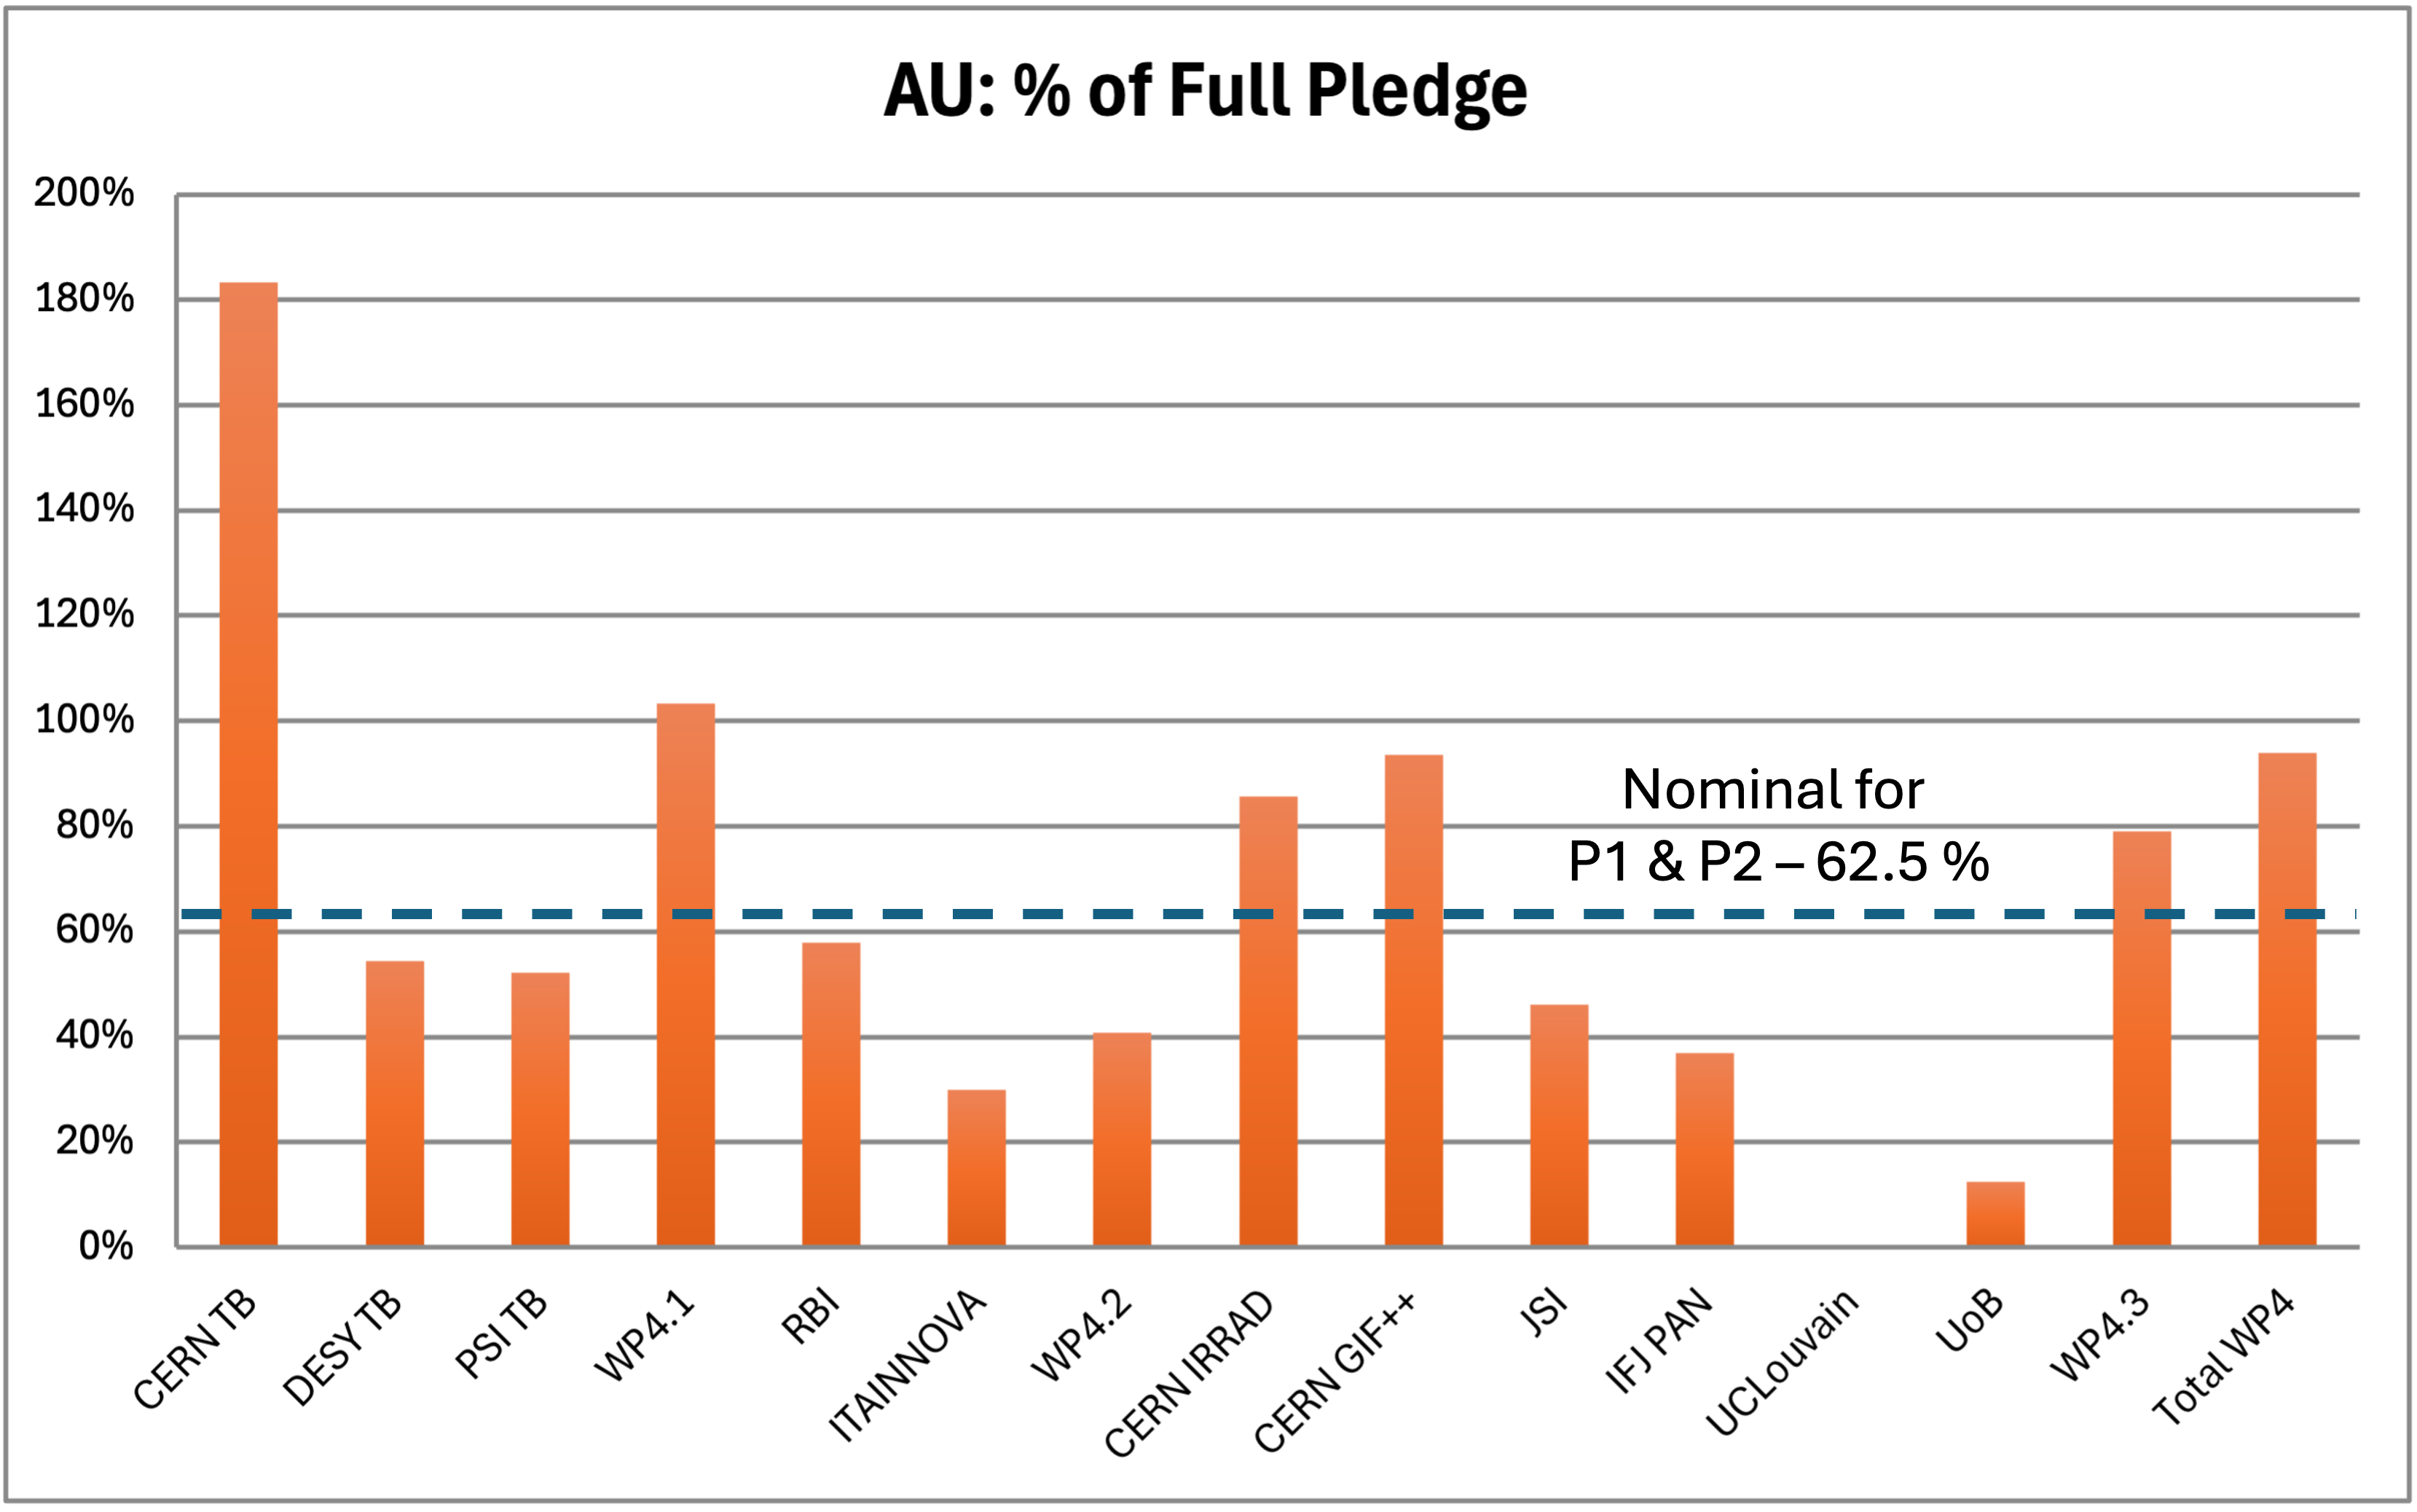
\includegraphics[width=0.75\linewidth]{AU_P12-pledge.png}
    \caption{Delivery of AUs across RIs, tasks and complete WP4. The nominal value for M30 of the project of 62.5\% is ploted as reference.}
    \label{fig:AUs}
\end{figure}

An analysis of more than 100 projects with over 400 users executed during P2 of EURO-LABS in RIs of WP4 reveals a great diversity of the users involved in experiments carried out within the TA framework. Based on the location of their institute  (Fig. \ref{fig:WP4-affiliation}) , the users come from 37 countries on four continents including an almost perfect coverage of EU member states. The distribution of user nationalities  (Fig. \ref{fig:WP4-nationality}) reveals their origin from 43 different countries. The gender balance (Fig. \ref{fig:WP4-gender}) with 21\% of female participation is not ideal, but somewhat typical for the field. The proportion of ECRs (Early Career Researchers), especially for the financially supported users, is very high due to intentional preference of funding students and post-docs.

\begin{figure}[!h]
    \centering
    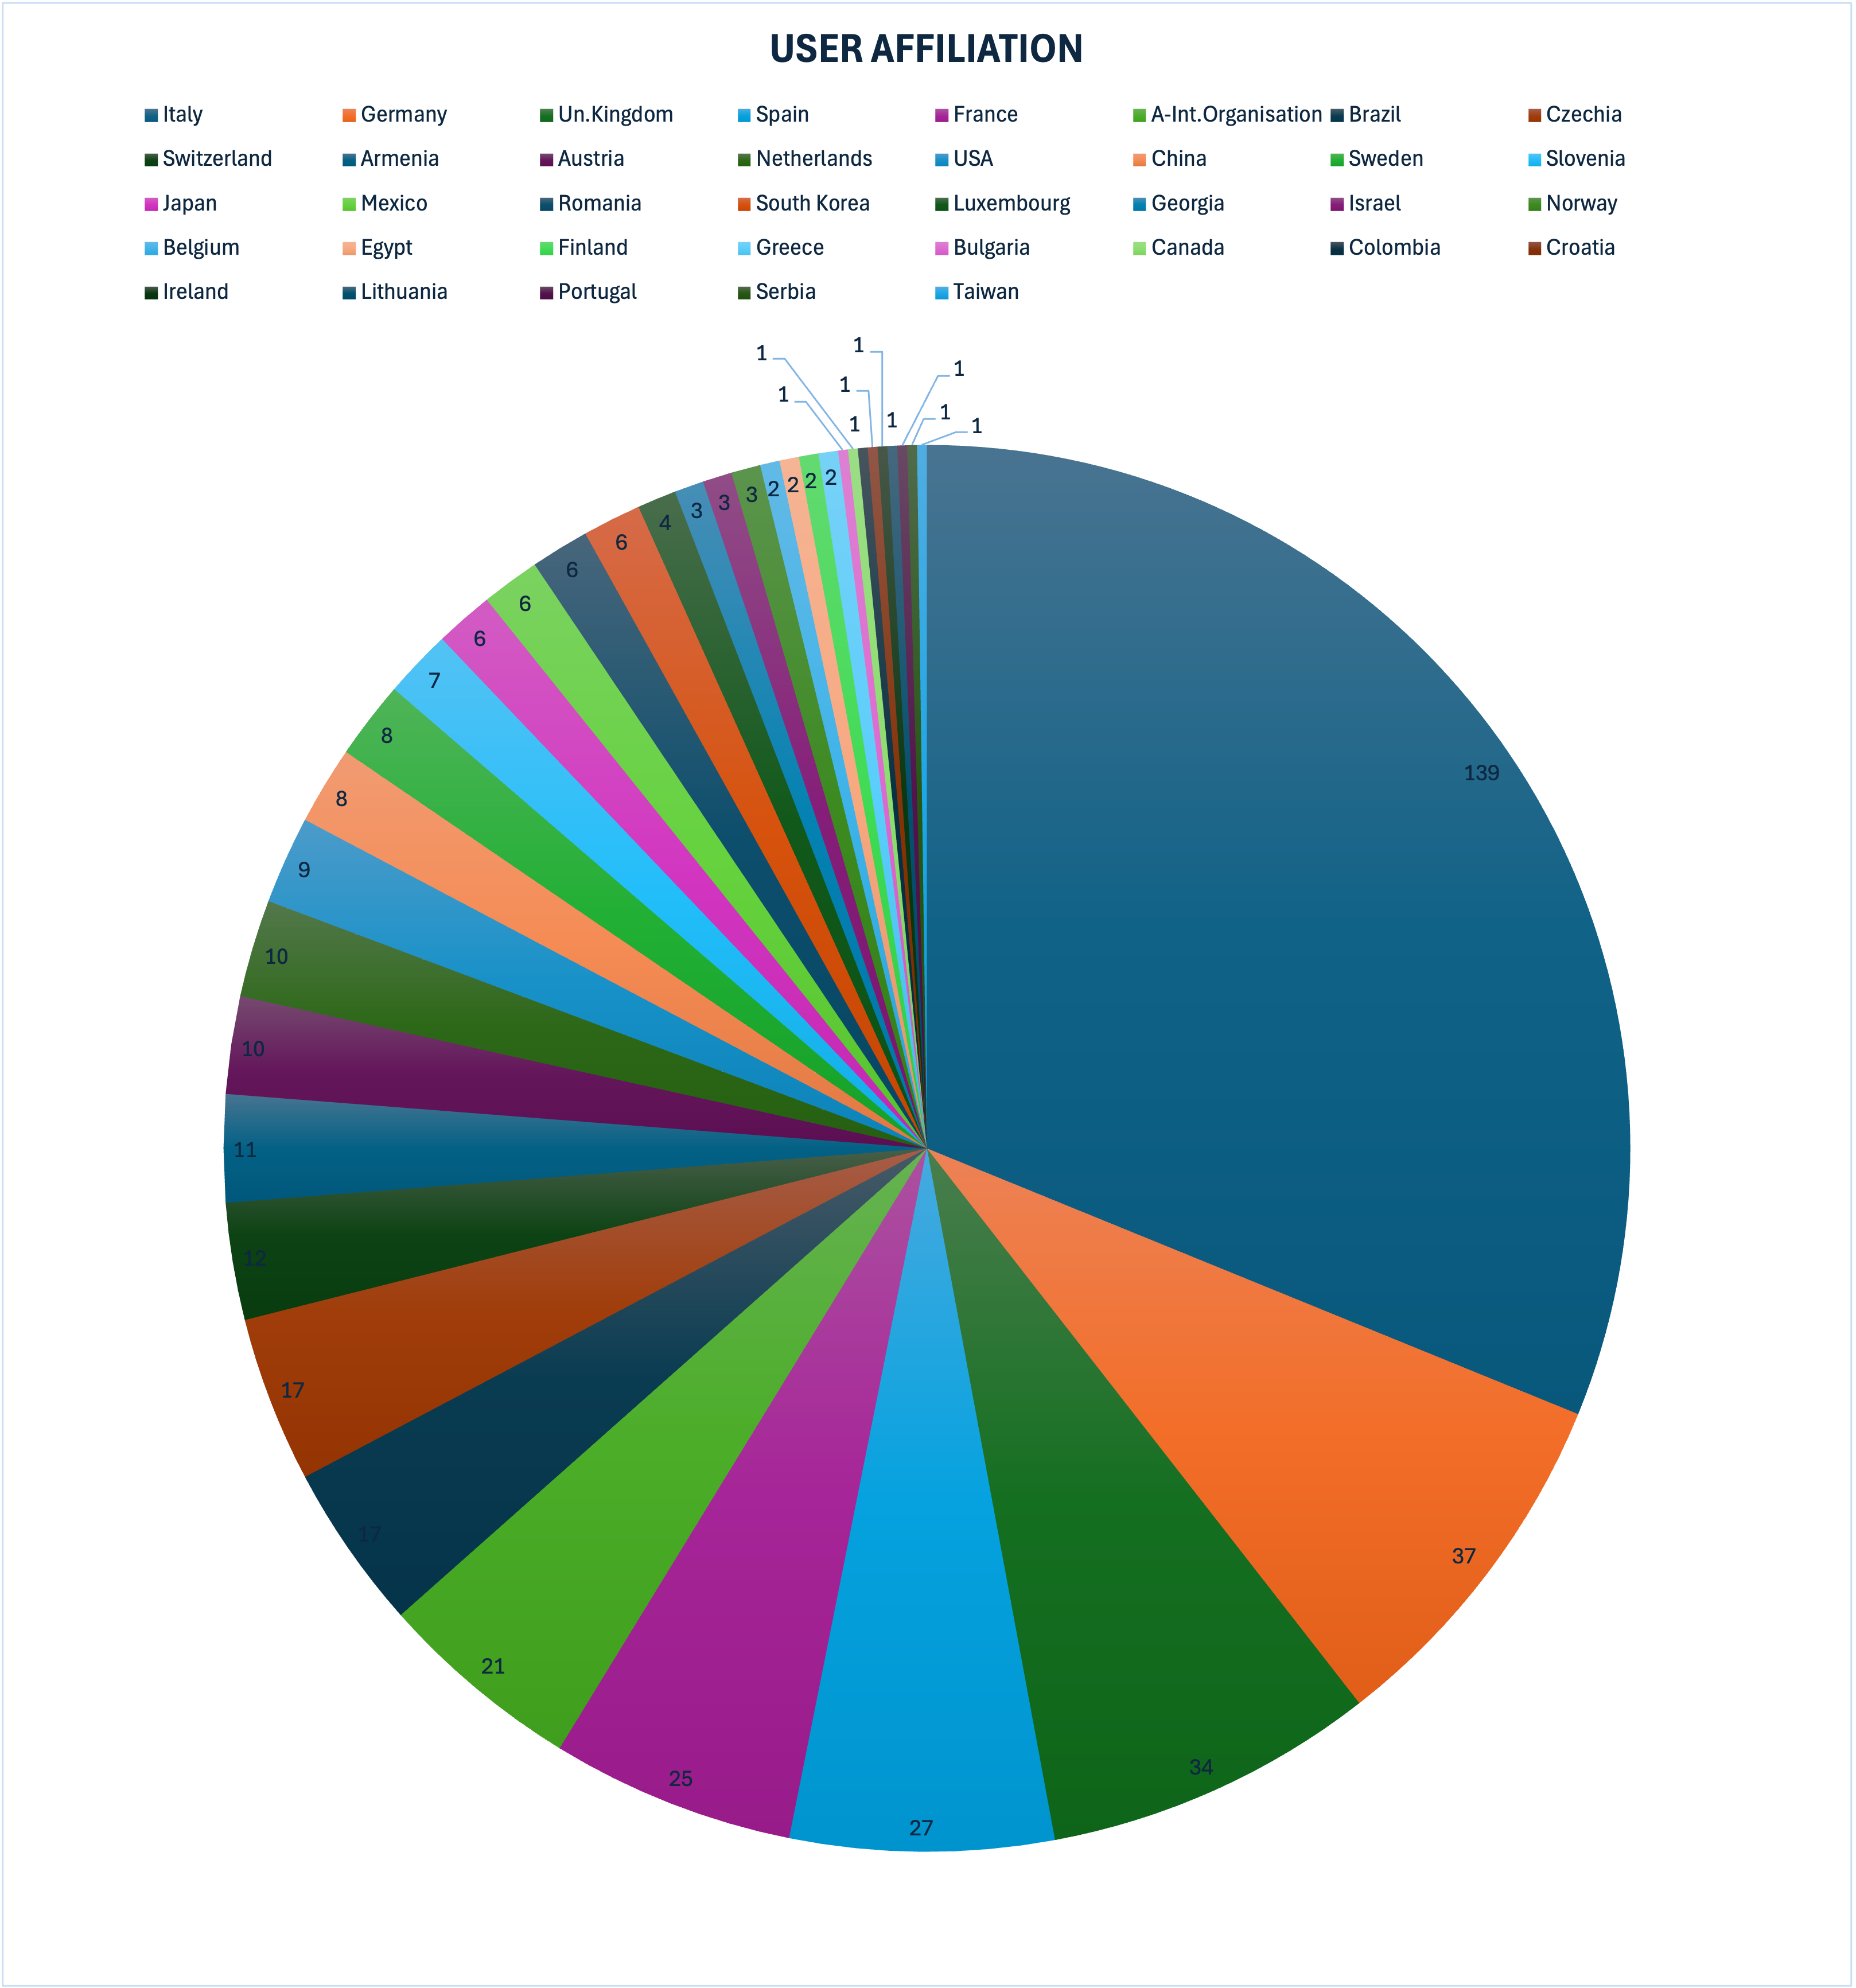
\includegraphics[width=0.75\linewidth]{P2-affiliation.png}
    \caption{Distribution of TA users in WP4 by country of affiliated institute in P2.}
    \label{fig:WP4-affiliation}
\end{figure}

\begin{figure}[!h]
    \centering
    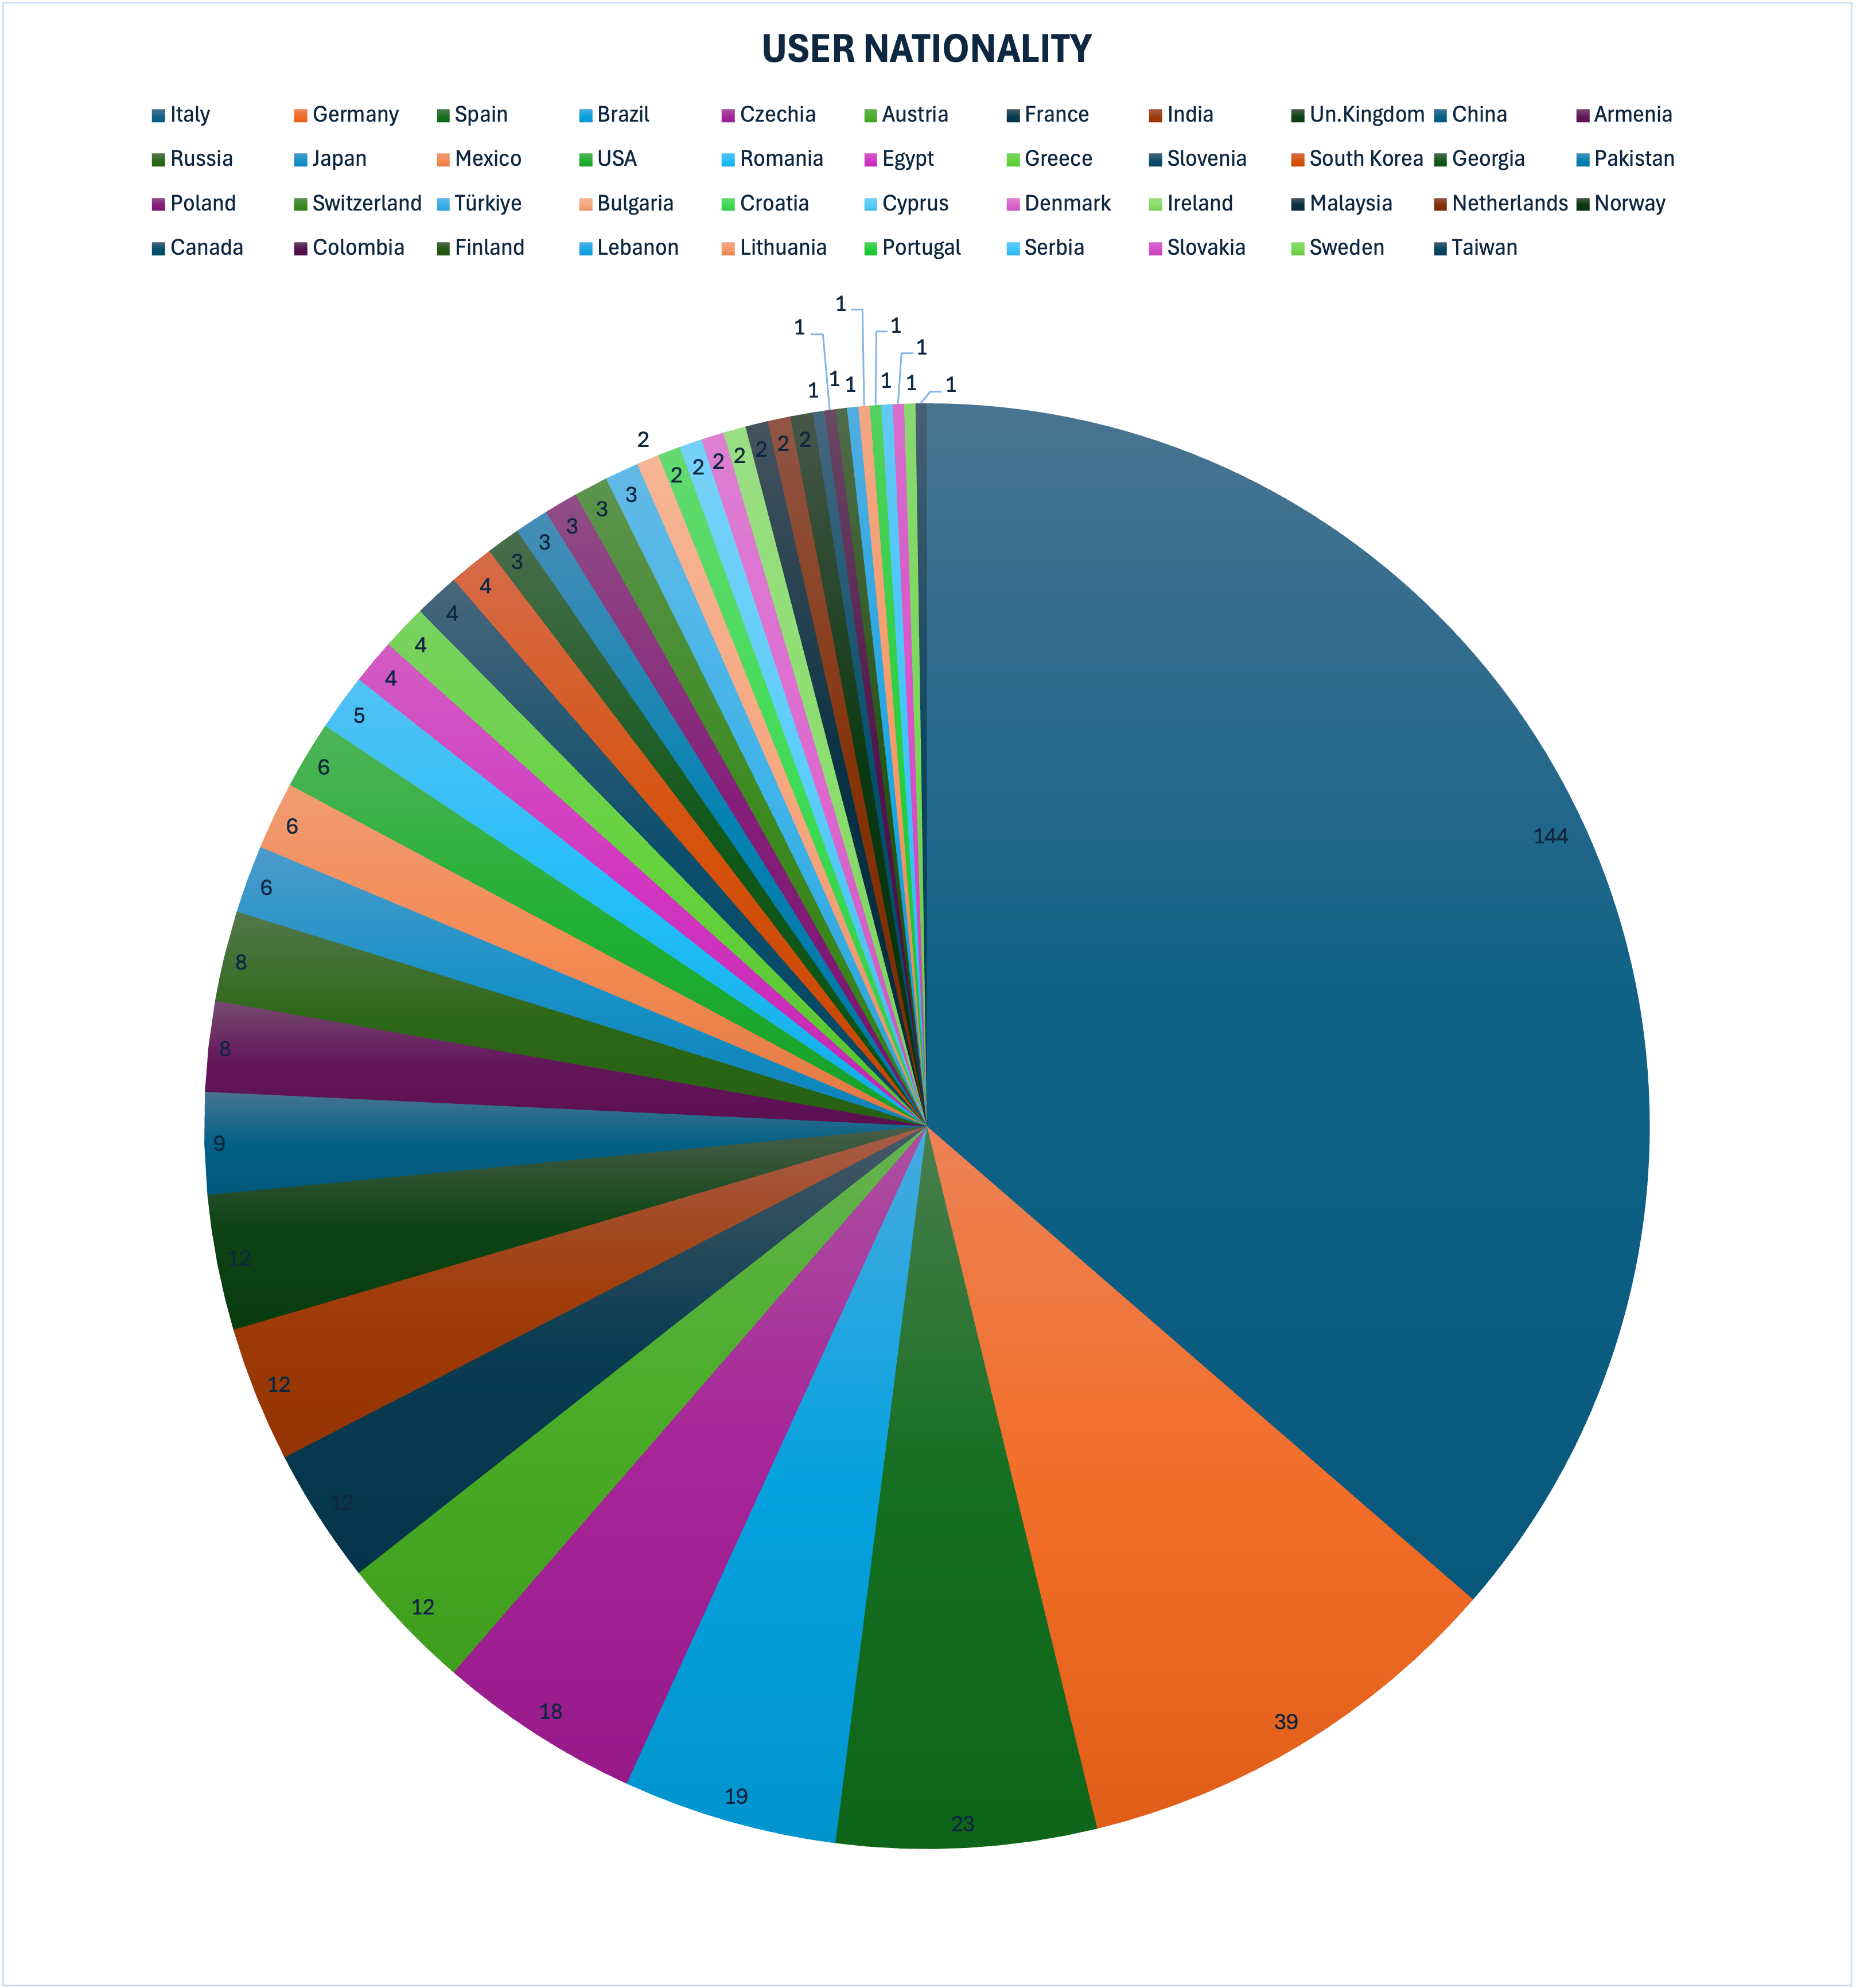
\includegraphics[width=0.75\linewidth]{P2-nationality.png}
    \caption{Distribution of TA users in WP4 by country of origin in P2}
    \label{fig:WP4-nationality}
\end{figure}

\begin{figure}[!h]
    \centering
    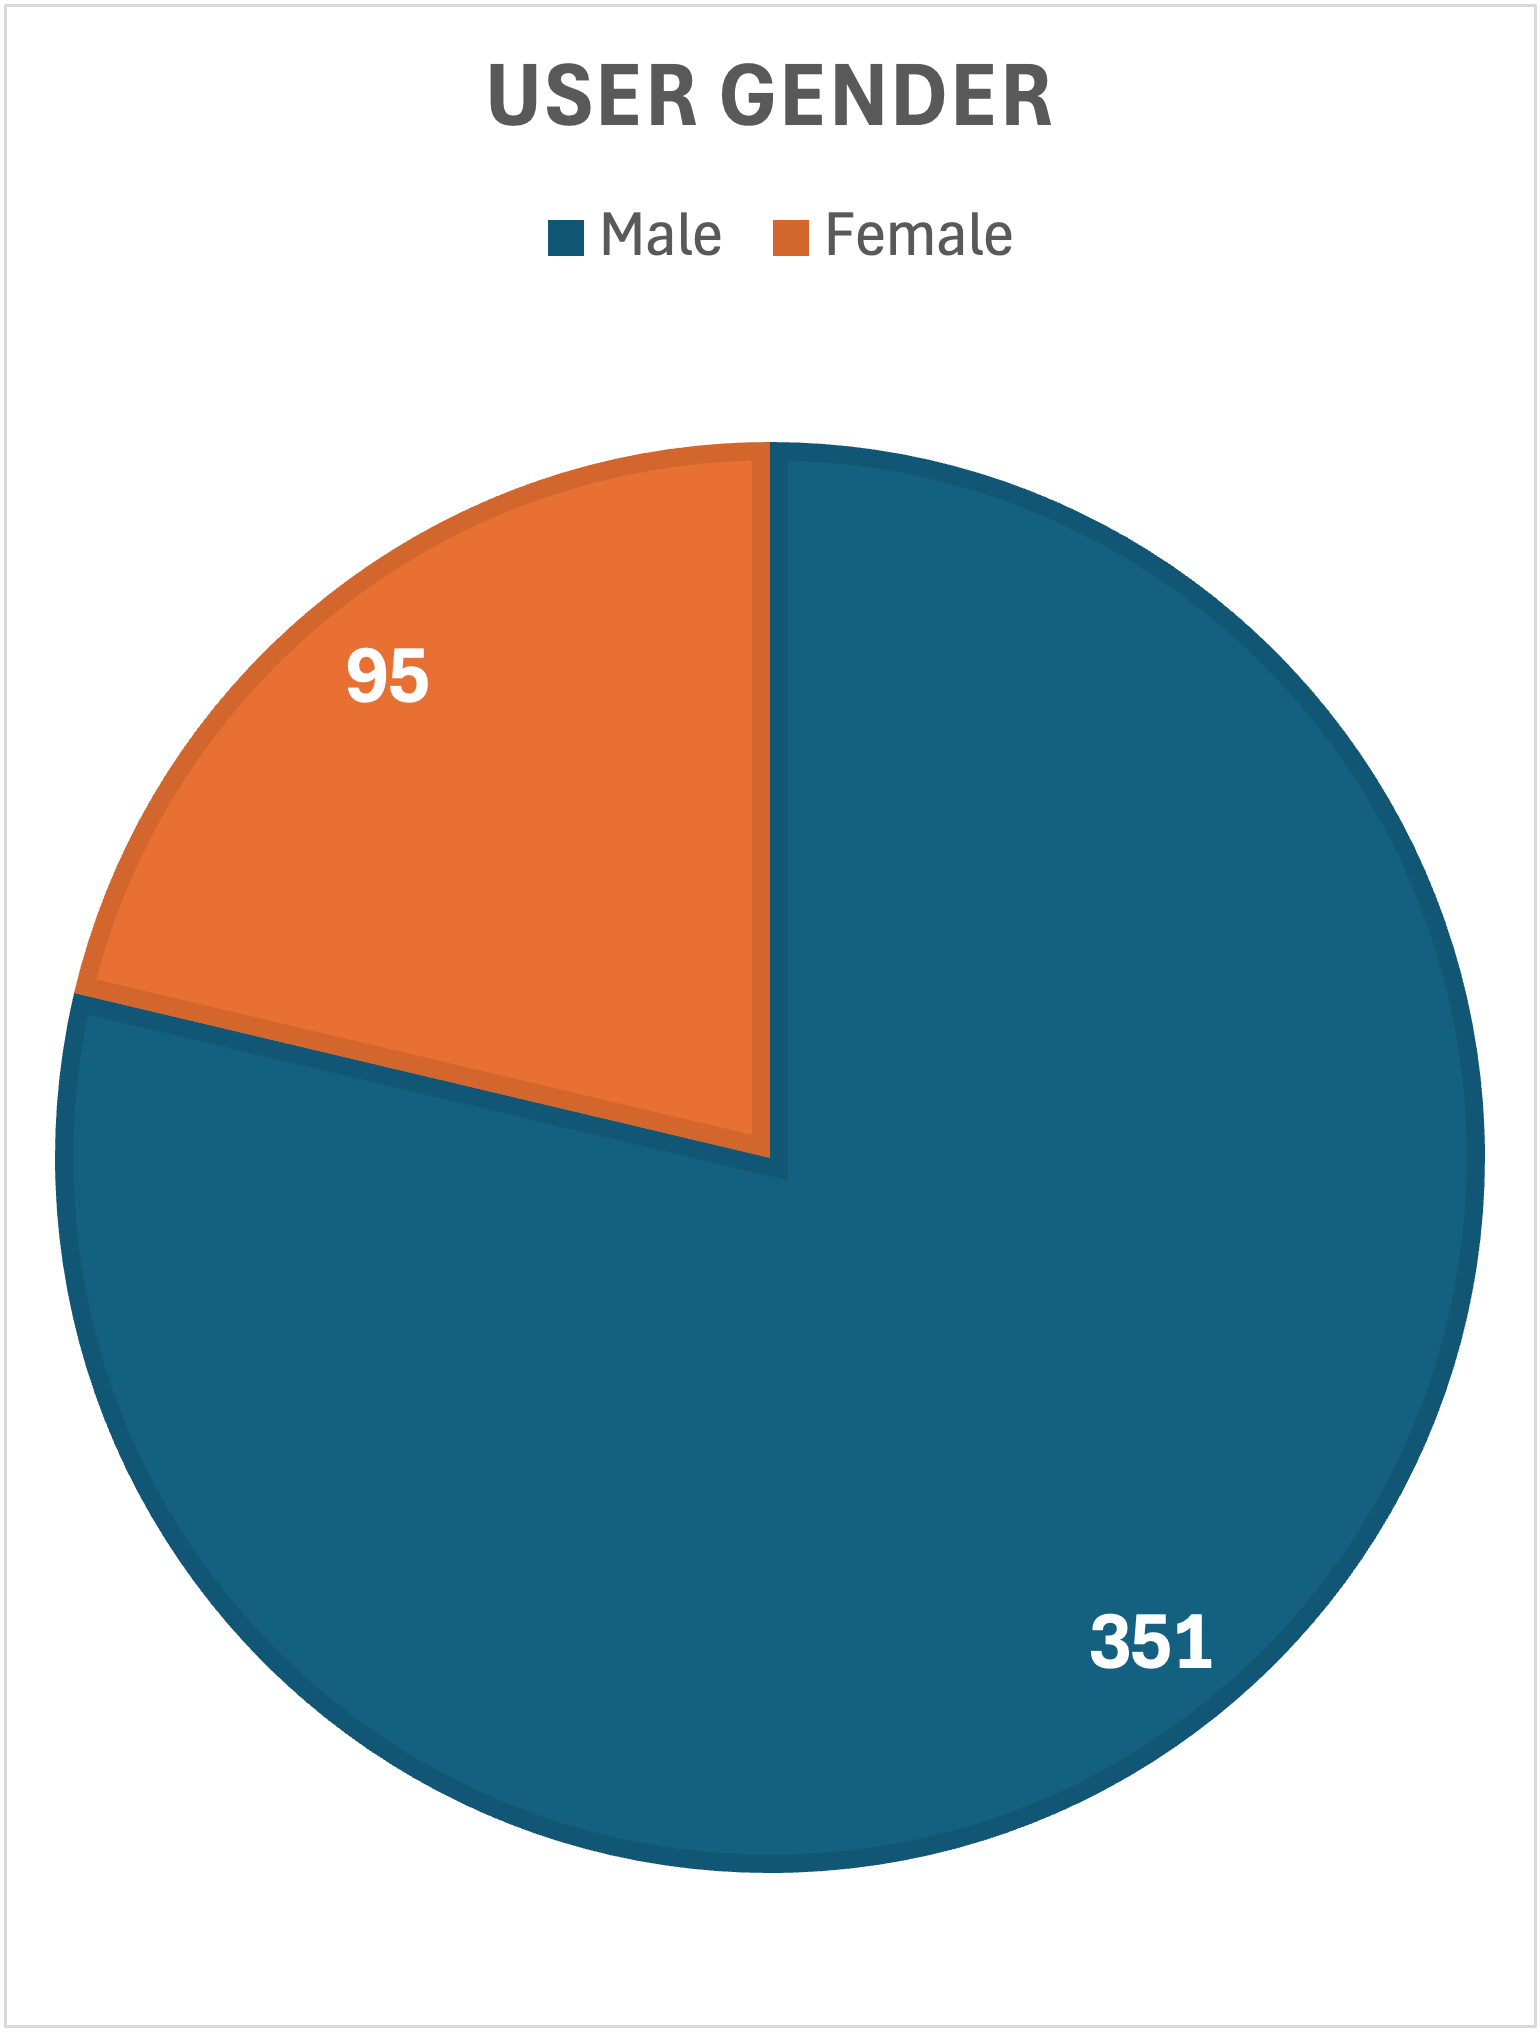
\includegraphics[width=0.5\linewidth]{P2-gender.png}
    \caption{Distribution of 446 WP4 users of TA by gender in P2.}
    \label{fig:WP4-gender}
\end{figure}

\subsubsection*{Deviations and Corrective Actions}
\label{sec:wp4_deviations}

In the remaining 18 months all the three RIs of WP4.1 can be reasonably expected to fulfil their pledge of AU in TA of EURO-LABS. While CERN has already done so, they will continue to deliver AUs to users interested in detector R\&D, as the updated accelerator schedule allows them to continue. DESY is keeping a steady pace towards their target and, barring unforeseen events, can be expected to continue this way. PSI, although experiencing a somewhat slower start, is catching up rapidly and, based on the substantial number of recently submitted applications, is also heading towards timely completion of its contribution.

Up to the end of the project, both RIs of WP4.2 can be expected to fulfil their pledge of AU. For RBI that involves keeping their pace; based on the flow of executed projects their user pool looks relatively stable. At ITTAINNOVA a larger effort is being made to persuade the builders of detector systems to conduct the tests of their detector assemblies at this unique facility. An investment needs to be made to educate the users of the advantages of those tests, best by presenting successful usage cases at internal meetings of the potential user communities.

Even with the overall goal of AU delivery achieved, the relatively meagre performance of some RIs of WP4.3 in delivery of AUs when compared to the nominal, pro-rata expectation calls for consorted action to ensure a successful completion of the project at all RIs. The temporal decline in user interest can be attributed to two facts: 
\begin{itemize}
\item The delays in the detector upgrades for the HL-LHC, which are binding a big pool of potential users to routine QA activities and solving problems that are not in line with genuine detector R\&D.
\item The organization of Detector R\&D (DRD) collaborations as the implementation of the ECFA Detector R\&D Roadmap. That process involved significant effort, effectively reducing the amount of R\&D activity. With all DRDC now in place, we can reasonably expect a boost in their detector R\&D activities. 
\end{itemize}
The construction of the upgrades is bound to last beyond the EURO-LABS project. There are still some modifications that can be regarded as pre-series verification and thus eligible for EURO-LABS support. The major upswing in user demand is though expected to arise from the activity of DRDs. DRD1 (gas detectors) has a large interest in GIF++, DRD3 (solid state) in all RIs (except GIF++) and DRD7 (electronics) in HIF and NIF at UCL (and possibly protons at IFJ-PAN). All the three DRDs were approached, delivering a presentation on EURO-LABS at their respective collaboration workshops. So, it is reasonable to expect an increased user demand for irradiation services, which should allow at task level but also individually at all the six RIs, the pledged amount of AUs to be reached.

\subsubsection*{Milestones and Deliverables}

{\fontsize{9}{11}\selectfont
\begin{center}
  \begin{tabular}[t]{!{\color{mygray}\vrule}p{0.10\linewidth}!
  {\color{mygray}\vrule}p{0.60\linewidth}!
  {\color{mygray}\vrule}p{0.20\linewidth}!{\color{mygray}\vrule} } \hline
    \rowcolor{mycyan} & {\bf Title} & {\bf Status} \\ \hline
    \cellcolor{mycyan}{\bf MS21}: & 4.1 - More than 30\% of AU delivered &  Achieved \\ \hline
    \cellcolor{mycyan}{\bf MS22}: & 4.2 - More than 30\% of AU delivered &  Achieved \\ \hline
    \cellcolor{mycyan}{\bf MS23}: & 4.3 - More than 30\% of AU delivered &  Achieved \\ \hline
    \cellcolor{mycyan}{\bf MS25}: & 4.4.3 	Prototype and software ready for lab tests &  Achieved \\ \hline
    \cellcolor{mycyan}{\bf MS26}: & 4.4.4 	Electrostatic Microprobe Quadrupole Quadruplet Lens Assembly installed and tested &  Achieved \\ \hline
    \cellcolor{mycyan}{\bf MS27}: & 4.4.5 	Cooling system developed &  Achieved \\ \hline
    \cellcolor{mycyan}{\bf MS29}: & 4.4.6 ML-based classification and evaluation of the beam profile patterns &  Achieved \\ \hline
    \cellcolor{mycyan}{\bf MS30}: & 4.4.7 	Design of the shielding system including safety related aspects &  Achieved \\ \hline
    \cellcolor{mycyan}{\bf MS31}: & 4.4.8 	Design of the XY table and purchase of materials and equipment for the device &  Achieved \\ \hline
    \cellcolor{mycyan}{\bf MS32}: & 4.4.10 Mechanics of the setup adapted to fit into the experimental area &  Achieved \\ \hline

  \end{tabular}
\end{center}
}

\subsubsection*{Project Meetings}
\begin{table}[H]
    \centering
    \caption{Summary of WP4-specific meetings in P2.}
    \begin{tabularx}{\textwidth}{|c|c|c|X|} \hline
        \rowcolor{mycyan}
        \textbf{Date} & \textbf{Meeting} & \textbf{Place} & \textbf{URL} \\ \hline
        18/9/2023 & WP4 quarterly meeting & Zoom & https://agenda.infn.it/category/1607/ \\ \hline         10/10/2023 & WP4 meeting during SAM & Krakow & https://agenda.infn.it/event/34651/ \\ \hline 
        25/3/2024 & WP4 quarterly meeting & Zoom & https://agenda.infn.it/category/1607/  \\ \hline        15/7/2024 & WP4 quarterly meeting & Zoom & https://agenda.infn.it/category/1607/ \\ \hline 
        29/10/2024 & WP4 meeting during TAM & CERN & https://indico.cern.ch/event/1370378/ \\ \hline 
        20/1/2025 & WP4 quarterly meeting & Zoom & https://agenda.infn.it/category/1607/ \\ \hline
     \end{tabularx}
    \label{tab:meetings}
\end{table}
%  {\color{mygray}\vrule}p{0.40\linewidth}!

%%%%%%%%%%%%%%%%%%%%%%%%%%%%%%%%%%%%%%%%%